In recent years, there has been a substantial increase in interest of open source projects. Open source software is typically developed by community of people interested in the particular area who do not necessarily know each other. These communities are usually web-based. Open-source phenomenon raises many interesting questions. Its proponents regard it as a paradigmatic change whereby the economics of private goods, built on the scarcity of resources, is replaced by the economics of public goods, where scarcity is not an issue. \cite{alexander2002working} There are many projects which are on top of their game and yet still being open source. For example, Apache, a free server program is often a go-to decision when web server implementation is needed. In 2002 it was used on 56\% of web servers worldwide \cite{lerner2001open}.

\section{History of Open-Source Software}
When talking about open source, most people immediately think of Linux. But there's so much more than than. The origin of open-source software can be traced back to the 1950s and 1960s, when software was sold together with hardware, and macros and utilities were freely exchanged in user forums. \cite{alexander2002working} In late 1983, GNU project has been announced and the next year a Free Software Foundation has been founded - both by an MIT employee Richard M. Stallman. All software written and released under Free Software Foundation had zero licences. The Linux kernel was released as freely modifiable source code in 1991 and like Unix, it attracted attention from many volunteer programmers. Another big milestone was a year 1998 when Netscape released a source code for Mozilla. In 1999 it was obvious that more and more corporate money will be invested into open source space as IBM announced their support for Linux by investing \$1 billion in its development.

\section{Types of Open-Source Software analysis}
Open-Source space is very interesting space to analyse. Not only because it was not that long ago, when a thought of decentralized team working on software for free seemed unlikely and now it is a common scenario, but also because of its nature. It does not hide anything and therefore all the data for the deeper analysis of requirements needed to success are up there for grabs. 
To determine whether an OSS project is thriving and sustainable, various analysis types can be done. The most obvious metric to look at is code activity and release history. This can be easily investigated by looking at projects' revision control system and pattern of contributions. Number of contributions usually differs as projects go through cycles of releases and cooldown periods. It's also hard to generalize between projects as they all have different approach towards releasing frequency. This is exactly the topic I'm studying in chapters \ref{ssec:crossCorrelation} and \ref{ssec:crossCorrelationCommits}.  Another important and also easier to interpret aspect is user community developed around the project/framework. Just a straightforward use of search engine statistics can show how popular various repositories are. This next point is little bit counter-intuitive, but healthy project should also have a reasonable number of known issues as it shows there is a real community behind the project using it. Therefore are bug tracking systems great source of information as well. Last but not least indicator and area to analyse project's success is the ecosystem as a whole. Seeing consultancy and customisation services or and companies that bundle the software with other products as part of solutions is a strong indicator the project is doing well.

\section{Choosing projects of interest}
There are loads of OSS projects nowadays and it turned out to be pretty interesting process to choose the best ones for my thesis. To make sure chosen projects fit into my work and fit  all my needs I defined several requirements which needed to be fulfilled at least to some extent:

\begin{itemize}
  \item Project needs to be widely used and well-known. This ensures there will be enough data on social media about it what will result in the less biased final results.
  \item Project has to have accessible bug tracking system or Git repository with list of known issues. This will provide the data for linking of social media with their corresponding GitHub issues.
  \item Ideally, projects could be from the same area to avoid coincidentally choosing an outlier project from some either popular or unpopular field.
\end{itemize}

After considering these three points, I ended up choosing several open source web development frameworks as my projects of interest. \\
Projects of my choice are NodeJS, AngularJS, EmberJS, VueJS for front-end technologies and Laravel, Symfony and CakePhp for backend PHP technologies. Some frameworks like  React, Meteor or Django have been left out because of their misleading names  would require lot of additional work to filter out data unrelated to the actual frameworks. For example, when tested Django framework, most of the twitter data referred to movie "Django Unchained".

\section{GitHub mining}
GitHub as a most-popular version control system is often a go-to choice for many OSS projects. With over 10 million repositories, it is becoming one of the most important source of software artifacts on the Internet \cite{russell2013mining}. Git providing valuable information and insight into projects happened to be the case in this thesis.\\
Thanks to GitHub Rest API v3\footnote{https://developer.github.com/v3/?} is data mining with GitHub very easy and straightforward. To send request to this API, OAuth2 token needs to be present in the request header. There are several ways how to acquire this token. I have decided to register an OAuth2 App under my GitHub account and that way I got constant token. Another way is to request a token programmatically, but I thought it would be an unnecessary overhead. OAuth2 applications can be registered under \textit{Account settings \textgreater Developer settings \textgreater Personal access tokens \textgreater Generate new token}.
\subsection{Release dates} \label{ssec:gitReleaseDatesMining}
To get the project release dates, I've sent one request to the endpoint \textit{git/refs/tags} (Listing \ref{lst:gitTagsEndpoint})

\begin{lstlisting}[caption={Requesting all project tags git API tags endpoint},label={lst:gitTagsEndpoint},language=Python]
request = Request(projectUri + "/git/refs/tags")
request.add_header('Authorization', 'token \%s' \% token)
project = urlopen(request).read()
tags = json.loads(project)
\end{lstlisting}

To get the release dates, after obtaining all tags, one more request for every one of them was needed (Listing \ref{lst:gitTagsEndpoint2}). Path to release date field within response body as JSON is tag \textgreater  object \textgreater  url \textgreater  Send new request \textgreater  author \textgreater  date.
\newpage
\begin{lstlisting}[caption={Requesting tag details and accessing release date},label={lst:gitTagsEndpoint2},language=Python]
	for tag in tags:
		version = tag['ref']
		got_object = tag['object']
		detailedUrl = got_object['url']

		#request details of particular release
		request = Request(detailedUrl)
		request.add_header('Authorization', 'token %s' % token)

		#get the person responsible for the release
		repoReleaseDetails = json.loads(urlopen(request).read())
		tagger = repoReleaseDetails['author']

		#get the date of the particular release
		releaseDate = tagger['date']
\end{lstlisting}

I saved the release dates in simple text file, one per line. This code was later on changed (in subsection \ref{ssec:crossCorrelationCommits}) to include also number of commits per release.

After executing this step, I needed to divide frameworks into groups based on their releasing frequency. I ended up with 3 groups:
\begin{itemize}
\item{Seldom releasing frequency} - less than once per month
\item{Medium releasing frequency} - between one and 3.5 times per month
\item{Often releasing frequency} - on average more than 3.5 releases per month
\end{itemize}

Using these values as bounds for groups, projects were divided into their respective groups. Projects, release counts and average release frequency are in Table \ref{table:releaseGroupsCalculation}.

\begin{table}[H]
\centering
\begin{tabular}{| p{2cm}|p{2cm}|p{2.8cm}|p{1.8cm}|p{2cm}|}
 \hline
\textbf{Group} & \textbf{ Project }& \textbf{Release count} & \textbf{ Months }& \textbf{Frequency}\\
 \hline
  \multirow{4}{*}{Often}   & EmberJS & 266   & 76 & 3.5\\ 
    & VueJS &  209 & 45 & 4.64 \\ 
    & NodeJS & 440 & 100 & 4.4\\  
    & Symfony & 291 & 76 & 3.82\\ \hline 
  \multirow{4}{*}{Medium}   & AngularJS & 190   & 82 & 2.34\\ 
    & CakePHP & 289 & 104 & 2.77\\ 
    & Bower &  102 & 60 & 1.7\\   \hline 
  \multirow{4}{*}{Seldom}   & Gulp & 16 & 25 & 0.64\\ 
    & Yii & 41 & 59 & 0.69\\ 
    & Bootstrap &  42 & 72 & 0.58\\  \hline 
\end{tabular}
\caption{OSS projects grouped according to their releasing frequency}
\label{table:releaseGroupsCalculation}
\end{table}


\subsection{Issues} \label{ssec:issuesMining}
To get the project issues, I have used the endpoint \textit{issues}. It offers various parameters like state, labels, sort, direction or since date. I have decided to work just with closed issues and snippet where I am sending the request can be seen in Listing \ref{lst:issuesEndpoint}).

\begin{lstlisting}[caption={Requesting 100 closed issues},label={lst:issuesEndpoint},language=Python]
request = Request(projectUri + '/issues?state=closed&perpage=100&page=' + str(pageNum))
\end{lstlisting}

It is also worth noting here that GitHub's REST API v3 considers every pull request an issue so I had to identify and filter them out using their \textit{pullRequest} key. I'm saving all the data API provides but later work only with bug description and title.\\
During my later work, I have realized the amount of issues is just too big and broad and not every issue is a bug or even remotely similar to bug. That was when I have decided to filter the issues and keep only real bugs. For this I have used Git labels. Labels on GitHub help organize and prioritize work. They can be applied to issues and pull requests to signify priority, category, or any other information you find useful. There are two types of labels - default and custom. GitHub provides default ones in every new repository. All default labels can be seen in Table \ref{fig:defaultLabels} and can be used to create a standard workflow in a repository:

\begin{figure}[H]%
    \centering
	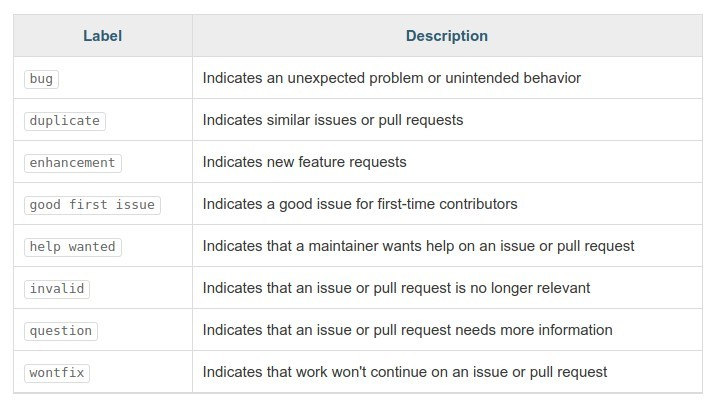
\includegraphics[width=11cm]{defaultLabels.jpg}
    \caption{Default Git labels provided for every repository}%
    \label{fig:defaultLabels}%
\end{figure}

From there I have chosen the label \textit{bug}. Then I have checked all custom tags of all repositories and chosen just those which were semantically similar to bug. All chosen labels can be seen in the Table \ref{table:allGitBugLabels}.


\begin{table}[H]
\centering
\begin{tabular}{ |p{3cm}||p{6cm}|}
 \hline
\textbf{ Repository }& \textbf{Chosen custom labels}\\
 \hline
 NodeJS   & confirmed-bug, errors \\ \hline
 AngularJS &   type: bug \\ \hline
 VueJS & browser-quirks, 1.x, 2.x\\ \hline
 Aurelia & enhancement\\ \hline
 EmberJS & Bug\\ \hline
\end{tabular}
\caption{Reddit submissions counts}
\label{table:allGitBugLabels}
\end{table}
